\chapter{Methods and ML/NN Algorithm Comparison}

\section{Aim and Evidential Standard}

This chapter describes the methodology used to compare conventional pulse-analysis methods with machine-learning and neural-network alternatives across the CCB test-beam programme. The central rule is deliberately conservative: no algorithmic result is considered interpretable until the raw-data population used by the original analysis has first been reproduced. In practice, each study begins from the B-stack ROOT branch \texttt{HRDv}, applies the S00 pulse gate, and verifies the selected-pulse count
\[
  A_{e,s}=\max_{k}\{x_{e,s,k}-\operatorname{median}(x_{e,s,0:3})\},
  \qquad A_{e,s}>1000~\mathrm{ADC},
\]
for the physical B staves B2, B4, B6, and B8. The full S00 population is \(640737\) selected B-stave pulse records, and representative downstream architecture studies reproduced not only this total but also the Sample-II analysis count \(125096\) and the per-stave counts B2 \(88213\), B4 \(21229\), B6 \(11148\), and B8 \(4506\).

The comparison target is not ``ML versus no ML'' in the abstract. For each physics question, the traditional comparator is the strongest available transparent method: amplitude-binned templates for waveform description, analytic amplitude timewalk for timing, bounded two-pulse fits for pile-up recovery, peak or integral calibrations for duplicate-readout closure, and leave-one-out pretrigger estimators for pedestal tests. The ML family is then evaluated only on train/test partitions that are disjoint in run number. This matters because run, current, calibration epoch, and topology are strong nuisance variables. A random row split would overstate generalisation.

\section{Run-Split Protocol and Metrics}

Let \(r(e)\) be the run number for event \(e\). Each benchmark defines disjoint sets \(\mathcal{R}_{\mathrm{train}}\), \(\mathcal{R}_{\mathrm{cal}}\), and \(\mathcal{R}_{\mathrm{test}}\), with
\[
  \mathcal{R}_{\mathrm{train}}\cap \mathcal{R}_{\mathrm{test}}=\varnothing .
\]
Hyperparameters are chosen using grouped cross-validation by run within \(\mathcal{R}_{\mathrm{train}}\), optional calibration uses only \(\mathcal{R}_{\mathrm{cal}}\), and the quoted number is evaluated once on \(\mathcal{R}_{\mathrm{test}}\). Event identifiers, run identifiers, event order, other-stave target quantities, and label-defining derived variables are excluded from the feature matrices unless the study is explicitly a leakage autopsy.

For timing residuals, the robust width is
\[
  \sigma_{68}(r)=\frac{1}{2}\left[Q_{0.84}(r)-Q_{0.16}(r)\right],
\]
where \(r\) is the held-out residual distribution. For amplitude or charge closure the primary resolution metric is
\[
  \mathrm{res}_{68}=\operatorname{quantile}_{0.68}
  \left(\left|\frac{\hat{y}-y}{y}\right|\right).
\]
For classifiers the primary ranking metrics are ROC AUC and average precision, with calibration checks such as Brier score when probabilities are used. Confidence intervals are non-parametric bootstrap intervals over the held-out unit appropriate to the claim: pulses or pair residuals for within-run precision, and run blocks when the conclusion is about transfer across runs.

\section{Leakage Controls and Fair Baselines}

The S07 rigour pass is the clearest example of the programme's guardrails. It asked whether waveform-shape features separate 2 nA low-current pulses from 20 nA high-current Sample-I pulses. The traditional method was not a strawman; inside each training fold it selected the best signed one-dimensional score from pre-registered pulse-shape candidates. The ML comparator was a calibrated random forest using normalized waveform samples and shape features, but no run id, current, stave id, absolute amplitude, hit multiplicity, or timing-derived labels. The run-held-out result is shown in Table~\ref{tab:s07-rigour}.

\begin{table}[H]
\centering
\caption{S07 run-held-out current/topology proxy benchmark. The ML model wins this weak-label ranking task, but the report explicitly does not interpret the score as a calibrated pile-up probability.}
\label{tab:s07-rigour}
\begin{tabular}{lccc}
\toprule
Method & ROC AUC & 95\% CI & Average precision \\
\midrule
Fold-local single-shape score & 0.504 & [0.491, 0.517] & 0.195 \\
Calibrated RF waveform-shape model & 0.768 & [0.758, 0.778] & 0.390 \\
ML minus traditional & 0.264 & [0.250, 0.280] & 0.195 \\
\bottomrule
\end{tabular}
\end{table}

The same rule also rejects attractive but invalid wins. Classifiers trained on \(D_t\), curvature, or other timing-control labels can reach AUC values near one because the target is a disguised function of the input timing construction. Those studies are retained as negative controls rather than promoted as detector conclusions. Conversely, injected waveform-corruption or artificial saturation labels are acceptable closure tests because the target is generated independently of the model features, even though such studies still require transfer caveats before production use.

\begin{figure}[H]
\centering
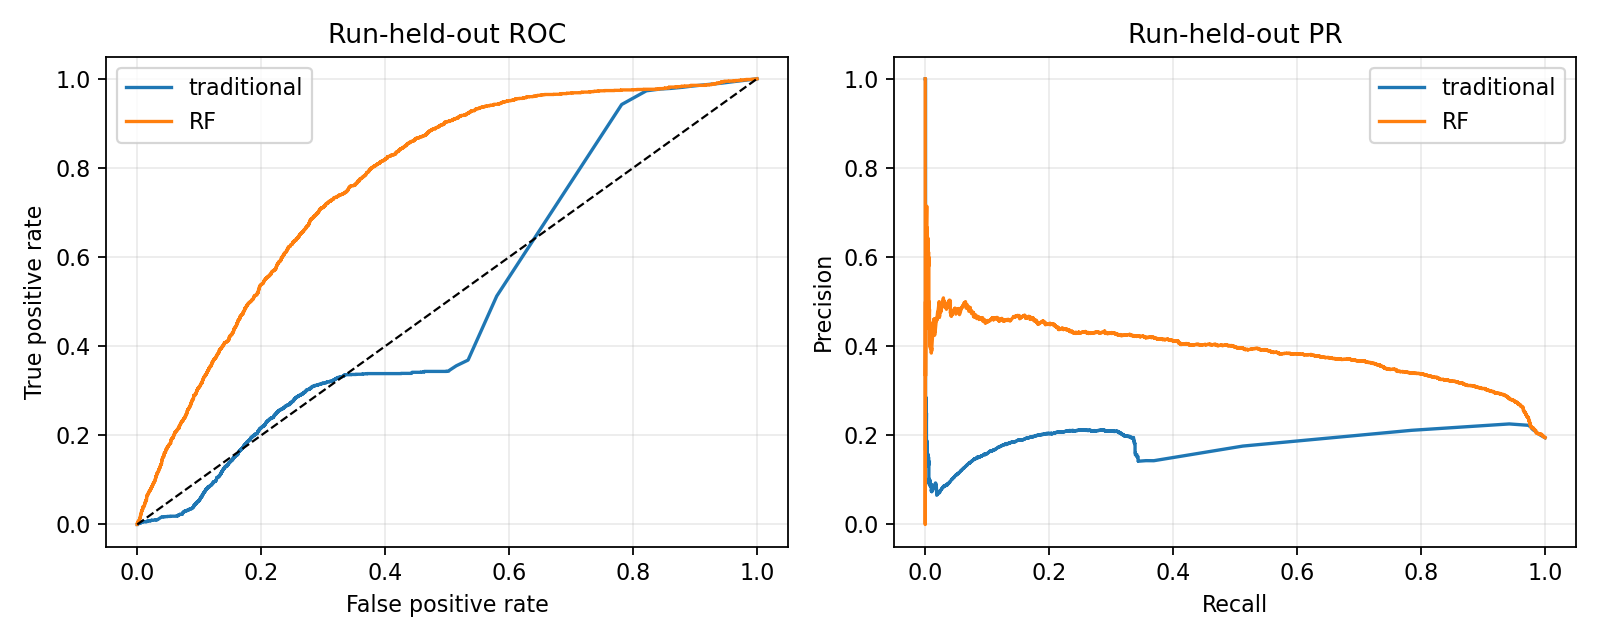
\includegraphics[width=0.78\linewidth]{../../reports/1780997954.15217.702122ea__s07_ml_rigour_scoreboard/fig_roc_pr.png}
\caption{S07 ROC/precision-recall comparison for the traditional shape score and calibrated waveform-shape random forest.}
\end{figure}

\section{Algorithm Families}

The algorithm set intentionally spans transparent linear methods, tree ensembles, and small neural networks. Ridge regression is used when the desired correction should be smooth, auditable, and low variance:
\[
  \hat{\beta}=\arg\min_{\beta}\sum_i (y_i-x_i^{T}\beta)^2+\lambda\|\beta\|_2^2 .
\]
Gradient-boosted trees and ExtraTrees are used for tabular waveform summaries where monotonicity is not guaranteed and local interactions matter. The neural set includes compact multilayer perceptrons, small one-dimensional convolutional networks, residual CNNs, temporal convolutional networks, attention blocks, and GRUs. The neural architectures are deliberately small because the waveform has only 18 samples; capacity is not the primary limitation unless the task includes longer time history or richer context.

The most systematic architecture comparison is S19a, the \texttt{nnarch} sweep. It used raw B-stack ROOT files, reproduced the S00 gate exactly, and evaluated two tasks: same-particle timing residual correction and injected two-pulse recovery. The timing baseline was the analytic amplitude-timewalk method; the two-pulse baseline was a bounded template fit. The ML/NN competitors included ridge, gradient-boosted trees, MLP, 1D-CNN, ResNet, TCN, attention, and GRU.

\section{Timing Architecture Bake-Off}

For timing, the corrected time is formed as
\[
  t'_{i,e}=t_{i,e}-x_i/v,
\]
and the per-pulse residual target is the deviation from the other downstream staves,
\[
  r_{i,e}=t'_{i,e,\mathrm{base}}-\frac{1}{2}\sum_{j\ne i}t'_{j,e,\mathrm{base}} .
\]
The strong traditional comparator is the analytic amplitude-timewalk correction. In the broad S19a architecture sweep, all learned models predicted only residuals left by this analytic baseline; no model received run id, event id, event order, other-stave times, or the held-out target.

\begin{table}[H]
\centering
\caption{S19a held-out timing architecture benchmark on run 65. Lower \(\sigma_{68}\) is better.}
\label{tab:timing-architecture}
\begin{tabular}{lccc}
\toprule
Method & Family & \(\sigma_{68}\) [ns] & 95\% CI [ns] \\
\midrule
MLP residual corrector & neural & 1.176 & [1.024, 1.386] \\
GRU residual corrector & neural & 1.225 & [1.014, 1.462] \\
Gradient-boosted trees & tree ensemble & 1.256 & [1.012, 1.438] \\
1D-ResNet & neural & 1.299 & [1.087, 1.497] \\
TCN & neural & 1.341 & [1.054, 1.560] \\
1D-CNN & neural & 1.363 & [1.030, 1.582] \\
Attention block & neural & 1.435 & [1.079, 1.632] \\
Ridge & linear ML & 1.443 & [1.196, 1.635] \\
Analytic amplitude timewalk & traditional & 1.495 & [1.299, 1.666] \\
S02 ridge-on-CFD20 & linear ML reference & 1.778 & [1.493, 2.070] \\
Template phase & traditional pickoff & 2.889 & [2.639, 3.277] \\
\bottomrule
\end{tabular}
\end{table}

The point-estimate winner is the MLP at \(1.176\) ns. The confidence interval for its improvement relative to the analytic baseline is negative, \(-0.319\) ns with CI \([-0.525,-0.060]\), so S19a names the MLP as the timing architecture winner for this screen. This conclusion is narrower than saying that neural networks generally solve timing. Earlier focused studies showed that a raw 18-sample MLP loses to the analytic baseline, and that a small CNN adds little when the residual target is already analytic-timewalk corrected. The current interpretation is that shallow nonlinear residual correction can help, but only after the physics timewalk term has carried most of the work.

\begin{figure}[H]
\centering
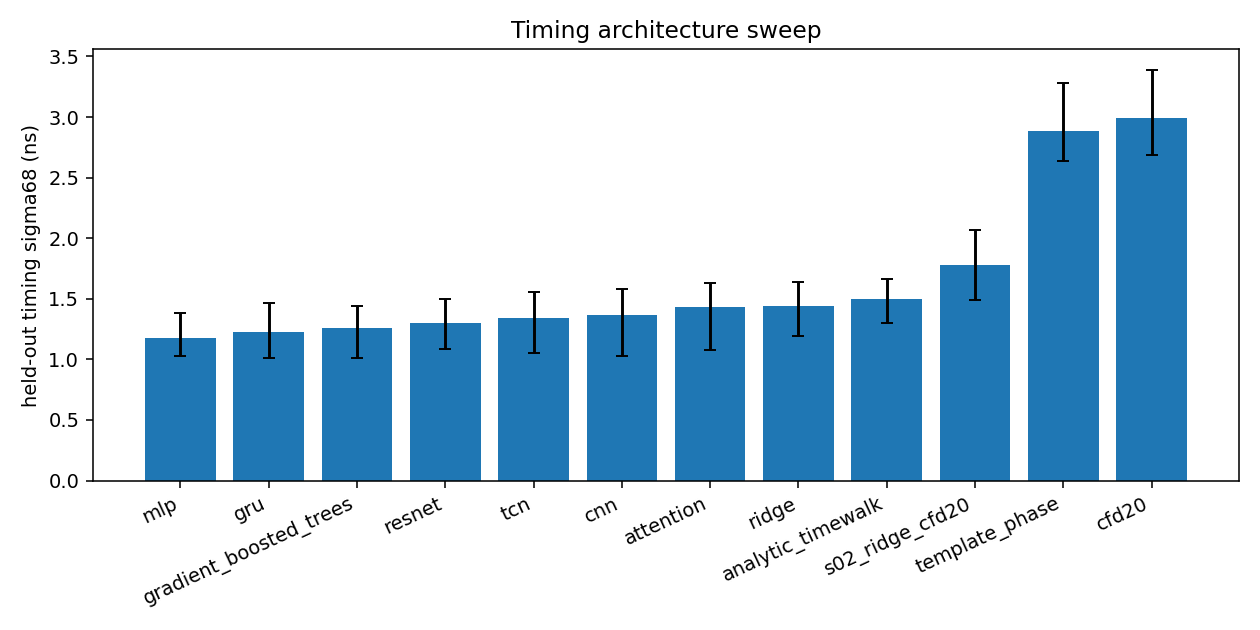
\includegraphics[width=0.82\linewidth]{../../reports/0000000006.1.nnarch__neural_architecture_sweep/fig_timing_architecture_sweep.png}
\caption{S19a timing architecture sweep. The MLP has the best held-out point estimate, while several more elaborate sequence architectures do not justify their extra structure on 18 samples.}
\end{figure}

\section{Two-Pulse Recovery Bake-Off}

The two-pulse task uses injected overlaps constructed from empirical templates and real residual pools. The traditional method scans constrained two-pulse hypotheses and solves amplitudes and baselines by least squares. The learned methods use waveform samples or same-channel waveform summaries to estimate overlap probability and recover two times and amplitudes. The target is synthetic but independent of the model features; it is therefore a method-ranking closure, not a measured real-pile-up truth label.

\begin{table}[H]
\centering
\caption{S19a held-out two-pulse architecture benchmark. Lower time RMS is better; AP and failure rate are guard metrics.}
\label{tab:twopulse-architecture}
\begin{tabular}{lcccc}
\toprule
Method & Family & AP & time RMS [ns] & failure rate \\
\midrule
Gradient-boosted trees & tree ensemble & 0.854 & 7.425 [7.402, 7.448] & 0.305 \\
Ridge/logistic heads & linear ML & 0.839 & 8.660 [7.886, 9.314] & 0.324 \\
MLP & neural & 0.814 & 10.435 [10.189, 10.662] & 0.324 \\
GRU & neural & 0.761 & 11.059 [10.581, 11.483] & 0.340 \\
1D-CNN & neural & 0.779 & 13.218 [12.704, 13.703] & 0.288 \\
TCN & neural & 0.726 & 13.248 [12.786, 13.665] & 0.314 \\
Constrained template fit & traditional & 0.775 & 13.874 [13.515, 14.222] & 0.155 \\
Attention block & neural & 0.707 & 13.985 [13.580, 14.343] & 0.355 \\
1D-ResNet & neural & 0.719 & 14.436 [13.550, 15.162] & 0.502 \\
\bottomrule
\end{tabular}
\end{table}

The point-estimate winner is gradient-boosted trees, with a time RMS of \(7.425\) ns compared with \(13.874\) ns for the bounded template fit. This agrees with earlier S10d and S11 closure tests in which compact ML reduced timing RMS or resolvability delay. The caveat is equally consistent: ML methods often pay for the lower RMS with a higher failure rate. The bounded template fit is less accurate on accepted events but safer operationally. Thus the algorithmic winner for injected recovery is gradient-boosted trees, while the production recommendation remains conditional on failure-rate control and real-current transfer.

\begin{figure}[H]
\centering
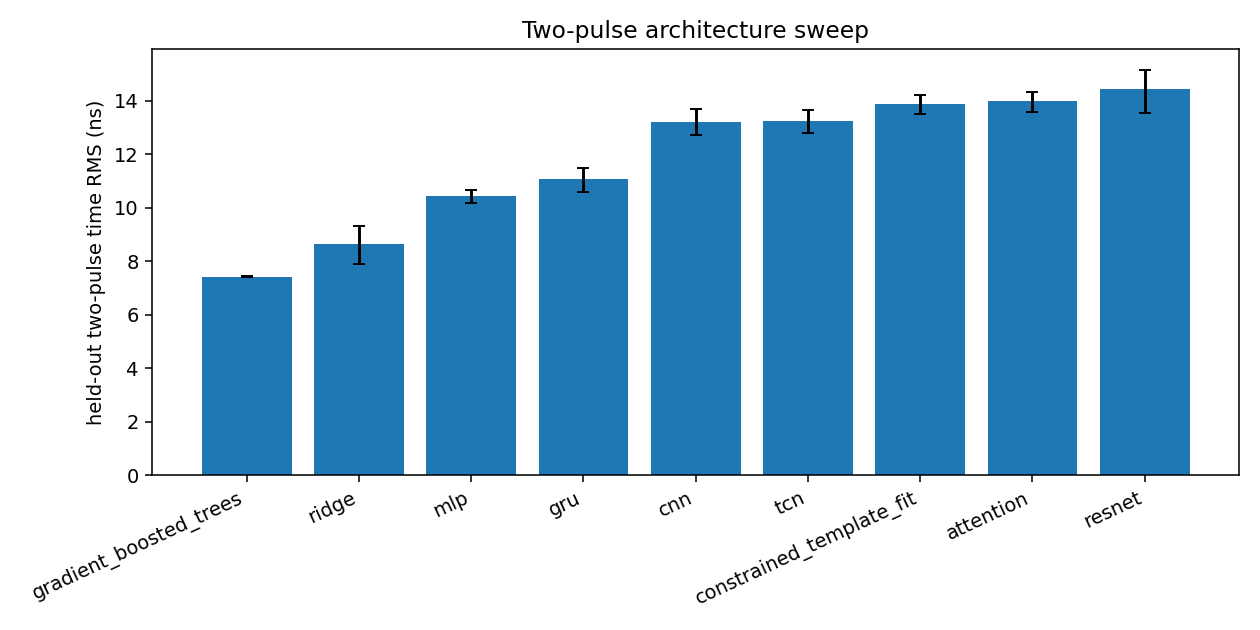
\includegraphics[width=0.82\linewidth]{../../reports/0000000006.1.nnarch__neural_architecture_sweep/fig_two_pulse_architecture_sweep.png}
\caption{S19a two-pulse architecture sweep. The tree model wins the injected closure by time RMS, while the traditional fit retains the lowest failure rate among the leading methods.}
\end{figure}

\section{Task-Level Winners Across the Programme}

The wider study programme shows a stable pattern. ML wins decisively when the independent target is encoded in waveform shape and the conventional baseline is too rigid. Traditional methods win or tie when the physics model is already close to sufficient, or when the proposed ML label is not independent of the input construction.

\begin{table}[H]
\centering
\caption{Representative task-level algorithm winners. Values are held-out or run-bootstrap results quoted in the individual reports.}
\label{tab:task-winners}
\begin{tabular}{p{0.19\linewidth}p{0.23\linewidth}p{0.23\linewidth}p{0.24\linewidth}}
\toprule
Task & Strong traditional method & ML/NN method & Winner and caveat \\
\midrule
Template reconstruction (S01) &
Amplitude-bin median template, MSE 0.0444 [0.0342, 0.0548] &
Autoencoder, MSE 0.00208 [0.00173, 0.00242] &
Autoencoder wins reconstruction; metric is shape residual, not timing truth. \\
\addlinespace
Compact representation (P02) &
PCA MSE 0.0262, 0.0142, 0.0088 for dims 2--4 &
Autoencoder MSE 0.0129, 0.0084, 0.0053 for dims 2--4 &
Autoencoder wins at dims 2--4; PCA wins by dim 8. \\
\addlinespace
Timing residuals (S19a) &
Analytic amplitude timewalk, \(\sigma_{68}=1.495\) ns [1.299, 1.666] &
MLP residual, \(\sigma_{68}=1.176\) ns [1.024, 1.386] &
MLP wins this architecture screen; analytic timewalk remains the essential baseline. \\
\addlinespace
Two-pulse recovery (S19a) &
Bounded template fit, RMS 13.874 ns [13.515, 14.222] &
Gradient-boosted trees, RMS 7.425 ns [7.402, 7.448] &
Trees win RMS; template fit has lower failure rate. \\
\addlinespace
Amplitude closure (P04) &
Peak calibration res68 0.1238; integral charge res68 0.1954 &
HGB res68 0.0091 amplitude; 0.0151 charge &
HGB wins duplicate-readout closure; not absolute energy truth. \\
\addlinespace
Saturation recovery (P07) &
Rising-edge template res68 0.104--0.286 &
GBR res68 0.032--0.046 &
GBR wins artificial clipping; natural saturation transfer remains systematic-limited. \\
\addlinespace
Pedestal proxy (S16) &
Mean3 MAE 260.7 ADC; adaptive MAE 341.0 ADC &
Calibrated HGBR MAE 48.9 ADC [43.8, 55.3] &
ML wins proxy target; no true forced/random pedestal sample is available. \\
\addlinespace
Conditional templates (P10b) &
Empirical template plus explicit timewalk, 2.756 ns [2.646, 2.868] &
Conditional MLP template, 3.579 ns [3.486, 3.680] &
Traditional explicit timewalk wins primary timing comparison. \\
\bottomrule
\end{tabular}
\end{table}

\section{Systematics and Caveats}

Several systematics recur across the algorithm comparisons.

First, the truth source determines what can be claimed. Duplicate odd-readout closure is an excellent target for waveform regression, but it is not an absolute deposited-energy label. Artificial clipping is a clean saturation benchmark, but it does not prove real saturated B2 truth. Injected overlaps rank two-pulse algorithms, but they do not by themselves measure the beam pile-up rate. Pretrigger leave-one-out targets expose pedestal bias, but they do not replace a forced/random-trigger pedestal sample.

Second, many apparent ML successes are actually target leakage tests. A classifier trained to identify a label derived from \(D_t\), curvature, or downstream residuals can learn the construction rather than a detector state. These results are valuable because they map unsafe labels; they are not promoted as physics measurements.

Third, confidence intervals do not cover every source of uncertainty. The bootstrap intervals quantify finite held-out statistics under a fixed model-selection procedure. They do not fully include architecture-search multiplicity, future run-domain shifts, real-current pathology missing from injected closures, or external calibration uncertainty. For this reason the reports separate ``point-estimate winner'' from ``production adoption''.

Fourth, the waveform length is short. The 18 samples contain enough local shape information for compact MLPs, tree ensembles, and occasional CNNs, but larger sequence architectures have not shown a robust advantage. In S19a, ResNet, TCN, attention, and GRU variants were sensible new architectures to try; none beat the simpler MLP on timing or the boosted trees on two-pulse recovery.

\section{Overall Algorithm Verdict}

Across the current programme, the best default is not a single model class. The correct hierarchy is:
\[
\begin{aligned}
&\mathrm{physics\ model}
\rightarrow \mathrm{strong\ transparent\ baseline} \\
&\rightarrow \mathrm{run\ split\ ML/NN\ residual\ or\ closure}
\rightarrow \mathrm{leakage\ and\ transfer\ audit}.
\end{aligned}
\]
Ridge is useful as a stable low-variance residual corrector and audit baseline. Gradient-boosted trees are the strongest general-purpose winners for tabular waveform closure and two-pulse recovery. MLPs can win timing residual screens when used after analytic timewalk. One-dimensional CNNs and larger sequence models are not broadly superior on these 18-sample pulses. The scientific conclusion is therefore nuanced: ML is most valuable for waveform-shape closure problems with independent targets, while traditional analytic methods remain the benchmark to beat for timing calibration and pile-up-rate interpretation.
